\documentclass[12pt,a4paper]{article}
\usepackage{verbatim}
\usepackage{amsmath}
\usepackage{graphicx}
\usepackage{float}
\author{ZHANG Xiao  research intern in IBM CRL}
\title{Network20q HW2}

\begin{document}
\maketitle
\pagebreak

\section{Ad space auction}
\subsection{a}
In the first question, we need to draw the bipartie graph and choose the maximum matching.

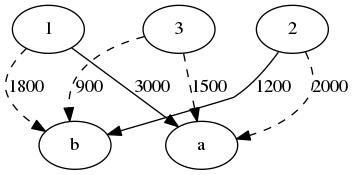
\includegraphics[width=\textwidth]{PIC/a.png}
The maximum matching could have the final solution: 1-A \$3000, and 2-b \$1200
\subsection{b}
The expected revenue vector of advertising 1,2,3 is
$
\begin{bmatrix}
    3000 \\
    1800
\end{bmatrix}
\begin{bmatrix}
    2000 \\
    1200
\end{bmatrix}
\begin{bmatrix}
    1500 \\
    900
\end{bmatrix}
$
respectively.
Then 1 would get A for the price of \$2000, and 2 would get B for the price of \$900.
So 1 would be charged \$4 per click, and receive payoff \$2 per click. Likewise, 2 would be charged \$3 per click, and receive payoff \$1 per click.

\section{Pagerank}
Because node 5 do not point to another node, 5 is a dangling node. So we need to use

$
\hat{H}=
\begin{bmatrix}
    0 & 1 & 0 & 0 & 0\\
    1 & 0 & 0 & 0 & 0\\
    1/3 & 0 & 1/3 & 0 & 1/3\\
    0 & 0 & 1/2 & 0 & 1/2\\
    1/5 & 1/5 & 1/5 & 1/5 & 1/5
\end{bmatrix}
$

And when $\theta = 0.1$

$
G= \theta \times \hat{H} + (1-\theta) \frac{1}{5} \times \vec{1} 
$

=
$
\begin{bmatrix}
0.18      &  0.28      & 0.18      &  0.18      &  0.18      \\
0.28      &  0.18     &  0.18      &  0.18      &  0.18       \\
0.21333333&  0.18      &  0.21333333&  0.18      &  0.21333333\\
 0.18      & 0.18    &  0.23    &  0.18     &  0.23     \\
0.2       &  0.2       &  0.2       &  0.2       &  0.2
\end{bmatrix}
$

Let $\pi = [1/5,1/5,1/5,1/5,1/5]^{T}$

We could calculate $\pi^{*} = \pi \times [G]^{n}$, when n is big enough. 

So we write a program to compare the recursive production of the multiplication of $\pi$ and $G$, when the norm between two steps is below 1e-6, the program stops. When $\theta = 0.1$, program stops at 5th step. And the $\pi^* = [ 0.21117058,  0.2051142 ,  0.19985902,  0.18399718,  0.19985902]$




when $\theta = 0.3$

$
G= \theta \times \hat{H} + (1-\theta) \frac{1}{5} \times \vec{1} 
$

=
$
\begin{bmatrix}
0.14&  0.44&  0.14&  0.14&  0.14\\
0.44&  0.14&  0.14&  0.14&  0.14\\
0.24&  0.14&  0.24&  0.14&  0.24\\
0.14&  0.14&  0.29&  0.14&  0.29\\
0.2 &  0.2 &  0.2 &  0.2 &  0.2
\end{bmatrix}
$

Let $\pi = [1/5,1/5,1/5,1/5,1/5]^{T}$

Program stops at 9th step. And the 

$\pi^* =[ 0.23789696,  0.22299348,  0.1937425 ,  0.15162455,  0.1937425 ]$




when $\theta = 0.5$

$
G= \theta \times \hat{H} + (1-\theta) \frac{1}{5} \times \vec{1} 
$

=
$
\begin{bmatrix}
0.1       &  0.6       &  0.1       &  0.1       &  0.1       \\
0.6       &  0.1       &  0.1       &  0.1       &  0.1       \\
0.26666667&  0.1       &  0.26666667&  0.1       &  0.26666667\\
0.1       &  0.1       &  0.35      &  0.1       &  0.35      \\
0.2       &  0.2       &  0.2       &  0.2       &  0.2
\end{bmatrix}
$

Let $\pi = [1/5,1/5,1/5,1/5,1/5]^{T}$

Program stops at 16th step. And the 

$\pi^* =[ 0.27450968,  0.25490208,  0.17647059,  0.11764706,  0.17647059]$



when $\theta = 0.85$

$
G= \theta \times \hat{H} + (1-\theta) \frac{1}{5} \times \vec{1} 
$

=
$
\begin{bmatrix}
0.03      &  0.88      &  0.03      &  0.03      &  0.03      \\
0.88      &  0.03      &  0.03      &  0.03      &  0.03      \\
0.31333333&  0.03      &  0.31333333&  0.03      &  0.31333333\\
0.03      &  0.03      &  0.455     &  0.03      &  0.455     \\
0.2       &  0.2       &  0.2       &  0.2       &  0.2
\end{bmatrix}
$

Let $\pi = [1/5,1/5,1/5,1/5,1/5]^{T}$

When $\theta = 0.85$, program stops at 62 step. And the 

$\pi^* = [ 0.39412997,  0.38032989,  0.09011066,  0.04531881,  0.09011066]$

The norm (distance) between two steps production is follows:

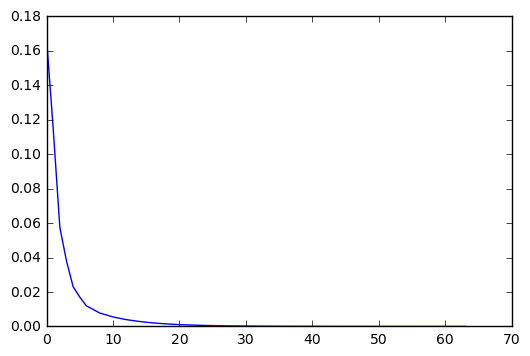
\includegraphics[width=\textwidth]{PIC/b.png}

From the result, we could conclude that: first, with the increase of $\theta$, the value of $\pi^*$ could use more steps to converge, and the distribution of the value could be more imbalanced.


\end{document}